\ifdefined\maindoc\else
% typesetting this chapter as a standalone document
\def\doctitle{ArtiSynth Overview}
\input{startdoc}
\mainmatter
\fi

\chapter{ArtiSynth Overview}
\label{Overview:sec}

ArtiSynth is an open-source, Java-based system for creating and simulating
mechanical and biomechanical models, with specific capabilities for the
combined simulation of rigid and deformable bodies, including finite element
(FE) models, together with contact and constraints. It is presently directed at
application domains in biomechanics, medicine, physiology, and dentistry, but
it can also be applied to other areas such as traditional mechanical
simulation, ergonomic design, and graphical and visual effects.

\section{System structure}

An ArtiSynth model is composed of a hierarchy of models and model components
which are implemented by various Java classes. Components are broadly divided
into {\it simulation components}, which include particles, rigid bodies,
springs, connectors, force effectors, individual finite elements, constraints,
etc., which are gathered together into {\it models} (including finite element
models), and {\it instrumentation components} such as control panels,
controllers and monitors, and input and output data streams (i.e., {\it
probes}), which have the ability to control and record the simulation as it
advances in time.  Instrumentation components are presented in more detail in
Chapter \ref{SimulationControl:sec}.

Every ArtiSynth component is an instance of
\javaclass[artisynth.core.modelbase]{ModelComponent}, while
components that contain subcomponents are instances of 
\javaclass[artisynth.core.modelbase]{CompositeComponent}.
A \javaclass[artisynth.core.modelbase]{ComponentList} is a {\tt
CompositeComponent} which contains a list of other components of a specific
type (such as particles, rigid bodies, springs, etc.).

All models and instrumentation components are collected together within a
top-level container known as a {\it root model}.  Simulation proceeds under the
control of a {\it scheduler}, which advances the models through time using a
physics simulator. A graphical user interface (GUI) allows users to view and
edit the model hierarchy, modify component properties, and edit and temporally
arrange the input and output probes using a {\it timeline} display.

\subsection{Simulation components}
%\label{ModelComponents:sec}
\label{SimulationComponents:sec}

Simulation components are those used to build a model or set of models to be
simulated. They are roughly divided into the following categories:

\begin{description}

\item[Dynamic components] \mbox{}\hfill\\ Components, such as
particles and rigid bodies, that contain position and velocity state, and
possibly mass. At present, dynamic components consist of
\javaclass[\mech]{Point}, \javaclass[\mech]{Frame}, 
and their subclasses. All dynamic components implement the Java interface
\javaclass[artisynth.core.mechmodels]{DynamicComponent}.

\item[Force effectors] \mbox{}\hfill\\
Components, such as springs or finite elements,
that exert forces between dynamic components.
All force effectors implement the Java interface
\javaclass[artisynth.core.mechmodels]{ForceEffector}.
Dynamic components are themselves also instances of {\tt ForceEffector}, since
they can exert velocity-based damping forces on themselves.

\item[Constrainers] \mbox{}\hfill\\
Components that enforce constraints between dynamic components. 
All constrainers implement the Java interface
\javaclass[artisynth.core.mechmodels]{Constrainer}.

\item[Attachments] \mbox{}\hfill\\
Components that can attach one dynamic component to another (see
Section \ref{ParametricAndAttached:sec}). While attachments are in principle the
same as constraints, they are implemented using a
different approach.  All attachment components
implement the Java interface 
\javaclass[artisynth.core.mechmodels]{DynamicAttachment}.

\item[Markers] \mbox{}\hfill\\
Subclasses of dynamic components which are always attached to other dynamic
components and contain the relevant attachment component internally.  All
currently implemented markers are subclasses of
\javaclass[\mech]{Marker} (attached points) and
\javaclass[\mech]{AttachedFrame} (attached frames).

\item[Visual components] \mbox{}\hfill\\
Components that provide graphical representation but do not actually affect the
simulation. Examples of these include mesh components that are not connected to
rigid bodies or FE models, and other implementations of 
\javaclass[artisynth.core.modelbase]{RenderableComponent} that are used for
visualization only.

\item[Models] \mbox{}\hfill\\
Composite components that agglomerate simulation components into a single
entity that contains state and can be advanced through time via the methods
{\tt initialize(t0)} and {\tt advance(t0, t1, flags)}, as discussed further in
Section \ref{ModelAdvancement:sec}. All models implement the Java interface
\javaclass[\mbase]{Model}. The primary model types used by
ArtiSynth are {\tt MechModel} (Section \ref{MechModel:sec}), which is the
primary container for a single mechanical or biomechanical model, and {\tt
RootModel} (Section \ref{RootModel:sec}), which combines one or more models
together with instrumentation components to form a loadable application model.

\end{description}

\subsection{The MechModel}
\label{MechModel:sec}

In most ArtiSynth applications, the simulation components 
used to construct the
model are collected under a single
\javaclass[artisynth.core.mechmodels]{MechModel}.
This is a 
\javaclass[\mbase]{Model} component that may
contain particles, rigid bodies, FE models, constraints, attachments, various
force effectors, and possibly other {\tt MechModel}s.  When a simulation is
run, the model's {\tt advance()} method invokes a physics simulator that
advances these components forward in time (Section
\ref{PhysicsSimulation:sec}).

For convenience each {\tt MechModel} contains a number of predefined
containers for different component types, including:

%\begin{framed}%
%\colorbox{shadecolor}{%
\begin{shadedregion}
\begin{tabular}{lll}
\hline
container name & description & component type \\
\hline
\tt particles & 3 DOF particles & dynamic \\
\tt points & other 3 DOF points & dynamic \\
\tt rigidBodies & 6 DOF rigid bodies & dynamic \\
\tt frames & other 6 DOF frames & dynamic \\
\tt frameMarkers & points which are attached to frames & marker \\
\tt axialSprings & point-to-point springs & force \\
\tt multiPointSprings & point-based springs with multiple via points & force \\
\tt frameSprings & 6 DOF springs between frames & force \\
\tt meshBodies & 3D surface mesh objects & visual \\
\tt connectors & joint-type connectors between bodies & constrainer \\
\tt constrainers & general constraints & constrainer \\
\tt forceEffectors & general force-effectors & force \\
\tt models & FE models and other MechModels & model \\
\tt attachments & attachments between dynamic components & attachment \\
\tt renderables & renderable components (for visualization only) & visual \\
\hline
\end{tabular}
\end{shadedregion}
Each of these is a child component of {\tt MechModel} and is
implemented as a
\javaclass[\mbase]{ComponentList}. Special methods
are provided for adding and removing items from them. 
If not used, the containers will simply remain empty.

\begin{sideblock}
Applications are not required to use these containers, and may instead create
any component containment structure that is appropriate, as described in
Section \ref{GeneralComponentArrangements:sec}.
\end{sideblock}

\subsection{Instrumentation components}
\label{InstrumentationComponents:sec}

Instrumentation components consist primarily of {\it control panels}, which
provide the ability to interactively adjust properties of simulation
components, and {\it simulation agents}, which are used to set inputs and
monitor outputs as a simulation proceeds
(Section \ref{ModelAdvancement:sec}). Both are described in detail in
Chapter \ref{SimulationControl:sec}.

\begin{description}

\item[Control panels] \mbox{}\hfill\\
GUI components that an application can create to interactively edit property
values of simulation components. They are described in
Section \ref{ControlPanels:sec}.

\item[Input probes] \mbox{}\hfill\\
Simulation agents that provide streams of input data to control the
simulation. Such data may include external force values, muscle excitation
levels, and position or velocity data for dynamic components which are being
controlled parametrically. Input probes work via an {\tt apply(t)} method,
which is called before each simulation step to determine the value of
the input data for time {\tt t} and (typically) use this to set
property values of simulation components associated with the probe.  They are
described in more detail in Section \ref{Probes:sec}.

\item[Controllers] \mbox{}\hfill\\
Simulation agents that perform computations, based on input probe data or the
state of the model, that are used to control the simulation.  As with input
probes, computed quantities typically include external forces, excitation
levels, and positions or velocities.  Computations are performed by an {\tt
apply(t0,t1)} method that is called before the simulation step between time
{\tt t0} and {\tt t1}. Controllers are often custom-defined by the application,
but predefined controllers (such as the inverse tracking controller described
in Chapter \ref{InverseSimulation:sec}) are also available. They are
described in more detail in Section \ref{ControllersAndMonitors:sec}.

\item[Monitors] \mbox{}\hfill\\
Simulation agents that compute simulation results, based on the state of the
model. These results can be directed to an output probe, saved to a specific
file, or just printed to the application console. Monitors are generally used
to compute quantities that are not explicitly available as properties within
the simulation components. Computations are performed by an {\tt apply(t0,t1)}
method that is called after the simulation step between time {\tt t0} and {\tt
t1}. Monitors are typically custom-defined by the application, and are
described in more detail in Section \ref{ControllersAndMonitors:sec}.

\item[Output probes] \mbox{}\hfill\\
Simulation agents that provide streams of output data to record the results of
the simulation. Such data may correspond directly to simulation component
properties, or to values computed by {\tt Monitor}s.  Common output probe data
includes reaction forces, contact pressures, and the position or velocity data
for dynamic components. Output probes work via an {\tt apply(t)} method, which
is called after a simulation step to determine and store the data for
simulation time {\tt t}; typically this data is determined from property values
of simulation components associated with the probe. Output probes are described
in more detail in Section \ref{Probes:sec}.

\end{description}

%Components which contain state information (such as position and
%velocity) should extend 
%\javaclass[\mbase]{HasState}, 
%which provides the methods
%\javamethod*[artisynth.core.modelbase.HasState]{getState()}
%and
%\javamethod*[artisynth.core.modelbase.HasState]{setState()}
%for saving and restoring state.
%
%A
%\javaclass[\mbase]{Model}
%is a sub-interface of {\tt CompositeComponent} and {\tt
%HasState} that contains the notion of advancing through time and which
%implements this with the methods {\tt initialize(t0)} and {\tt
%advance(t0, t1, flags)}, as discussed further in
%Section \ref{ModelAdvancement:sec}.
%The most common instance of {\tt Model} used
%in ArtiSynth is {\tt MechModel} (Section \ref{MechModel:sec}), which
%is the top-level container for a mechanical or biomechanical model.

\subsection{The RootModel}
\label{RootModel:sec}

The top-level component in the hierarchy is the {\it root model}, which is an
application-specific subclass
of \javaclass[artisynth.core.workspace]{RootModel} and which contains a list of
simulation models, along with containers for instrumentation components used to
control and interact with these models. The containers in {\tt RootModel}
include:

\begin{shadedregion}
\begin{tabular}{ll}
\hline
container name & description \\
\hline
\tt models & top-level simulation models of the component hierarchy \\
\tt inputProbes & input data streams for controlling the simulation \\
\tt controllers & functions for controlling the simulation \\
\tt monitors & functions for observing the simulation \\
\tt outputProbes & output data streams for observing the simulation \\
\tt controlPanels & application defined control panels for property editing \\
\tt renderables & renderable components (for visualization only) \\
\hline
\end{tabular}
\end{shadedregion}

Root models are created either by applications overriding the
root model's 
\javamethod[artisynth.core.workspace.RootModel]{build()}
method, or by reading the model directly from a {\tt .art} file
(Section \ref{LoadingAndRunning:sec}).

When a simulation is run, the root model's
\javamethod[artisynth.core.workspace.RootModel]{advance(,,)}
method is used to advance the simulation forward by a single time step. This
involves applying any input probes and controllers, calling the {\tt advance()}
method for each of the simulation models, and then applying any monitors
and output probes (Section \ref{ModelAdvancement:sec}).

\subsection{Component numbers, names and path names}
\label{PathNames:sec}

Whenever a component is added to the component hierarchy,
it is assigned a unique number relative to its
parent; the parent and number can be obtained using the methods
\javamethod[artisynth.core.modelbase.ModelComponent]{getParent()} and
\javamethod[artisynth.core.modelbase.ModelComponent]{getNumber()},
respectively.  Components may also be assigned a name (using
\javamethod*[artisynth.core.modelbase.ModelComponent]{setName()})
which is then returned using
\javamethod*[artisynth.core.modelbase.ModelComponent]{getName()}.

\begin{sideblock}
A component's number is not the same as its {\it index}.  The index
gives the component's sequential list position within the parent, and
is always in the range $0 \ldots n-1$, where $n$ is the parent's
number of child components. While indices and numbers frequently are
the same, they sometimes are not. For example, a component's number is
guaranteed to remain unchanged as long as it remains attached to its
parent; this is different from its index, which will change if any
preceding components are removed from the parent. For example, if we
have a set of components with numbers
%
\begin{verbatim}
0 1 2 3 4 5
\end{verbatim}
%
and components 2 and 4 are then removed, the remaining components will
have numbers
%
\begin{verbatim}
0 1 3 5
\end{verbatim}
%
whereas the indices will be {\tt 0 1 2 3}. This consistency of
numbers is why they are used to identify components.
\end{sideblock}

The names and/or numbers of a component and its ancestors can be used to form a
component path name. This path has a construction analogous to Unix file path
names, with the '/' character acting as a separator. Absolute paths start with
'/', which indicates the root model. Relative paths omit the leading '/' and
can begin lower down in the hierarchy. A typical path name might be
\begin{verbatim}
  /models/JawHyoidModel/axialSprings/lad
\end{verbatim}
For nameless components in the path, their numbers can be used
instead.  Numbers can also be used for components that have
names. Hence the path above could also be represented using
only numbers, as in
\begin{verbatim}
  /0/0/1/5
\end{verbatim}
although this would most likely appear only in machine-generated
output.

\section{Simulation overview}

An overview of the ArtiSynth simulation mechanism is given here.  More
details are given in \cite{lloyd2012artisynth} and in the related
\href{http://www.artisynth.org/doc/artisynth.pdf}{overview paper}.

\subsection{Model advancement}
\label{ModelAdvancement:sec}

ArtiSynth simulation works by advancing models forward in time using a series
of time steps, with a physics integrator updating positions, velocities and
forces for all of the dynamic components over each step.  The step size is
usually fixed, but {\it can} vary between models and also over different time
ranges, as described in more detail in the ``Advancing Models in Time'' section
of the
\artisynthManual{artisynth}{ArtiSynth Reference Manual}.

Simulation happens under the control of a {\it scheduler}, which determines the
next time to advance to and then advances the root model using its {\tt
advance()} method. In pseudo-code, this looks like:
%
\begin{lstlisting}[]
   double t0 = 0;
   while (simulating) {
      double t1 = getNextAdvanceTime (t0);
      rootModel.advance (t0, t1);
      t0 = t1;
   }
\end{lstlisting}
%
Most often, the next advance time is determined by adding the value of the root
model's {\sf maxStepSize} property to {\tt t0}.

\begin{figure}[ht]
\begin{center}
 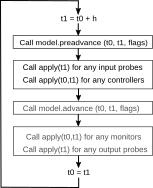
\includegraphics[width=3in]{images/modelAdvancement}
\end{center}
\caption{Typical model advancement sequence, from time $t_0$
to time $t_1$.}
\label{modelAdvancement:fig}
\end{figure}

Within its {\tt advance()} method, the root model in turn calls the {\tt
advance()} methods for its collection of models, while also calling the {\tt
apply()} methods for the model agents. For each model, the advancement sequence
typically looks like that shown in Figure \ref{modelAdvancement:fig}, with any
input probes and controllers called before the {\tt advance()} method and any
monitors and output probes called after. The {\tt preadvance()} method is an
additional method that a model can use to perform pre-step initialization
before input probes and controllers are called.

By default, the update interval $h$ in Figure \ref{modelAdvancement:fig} equals
the {\sf maxStepSize} of the root model. However, $h$ will be less if required
by the model's own {\sf maxStepSize} value, or a smaller (explicit) update
interval for any of the output probes. Figure \ref{modelAdvancement:fig} also
assumes that all of the model agents are explicitly associated with the
model. Input probes and controllers that are {\it not} associated with the
model will be applied {\it before} the {\tt preadvance()} method, and monitors
and output probes not associated with the model will be called after those that
are. Again, more precise details on this are given in the ``Advancing Models in
Time'' section of the \artisynthManual{artisynth}{ArtiSynth Reference Manual}.

\subsection{Full coordinate formulation}

It is important to understand that ArtiSynth uses a {\it full coordinate}
formulation, in which the position and velocity of each dynamic body is both
represented and solved using full, or unconstrained, coordinates, with extra
equations added to the system solve to account for constraints such as joints
and contact. In particular, point positions and velocities are represented
using 3-vectors, while the ``positions'' of {\tt RigidBody} and {\tt Frame}
components are represented as the translation and orientation of their
coordinate frames.  Internally, these frames are stored as a 3-vector plus a
quaternion, but they are most often presented to the application as the body's
{\it pose}, which is the $4 \times 4$ homogeneous transformation $\T_{BW}$ that
maps points from body to world coordinates:
%
\begin{equation*}
\T_{BW} =
\matl
\R_{BW} & \p_{BW} \\
0 & 1
\matr.
\end{equation*}
%
Here $\R_{BW}$ is a $3 \times 3$ rotation matrix and $\p_{BW}$ is a 3-vector
giving the location of the frame origin in world coordinates. The ``velocity''
of {\tt RigidBody} and {\tt Frame} components is the spatial velocity
%
\begin{equation*}
\hat\v_{BW} \equiv \matl \v_{BW} \\ \Bom_{BW} \matr
\end{equation*}
%
where $\v_{BW}$ and $\Bom_{BW}$ give the coordinate frame's translational and
angular velocity in world coordinates.  See Sections \ref{RigidTransforms:sec}
and \ref{SpatialVelocitiesAndForces:sec} for more details.

In contrast, some other simulation systems, including OpenSim
\cite{delp2007opensim}, use {\it reduced} coordinates, in which the system
dynamics are formulated using a smaller set of coordinates (such as joint
angles) that implicitly take the system's constraints into account.  For
example, a two degree-of-freedom (DOF) double pendulum in ArtiSynth is
described using 12 degrees of freedom (six for each of the two bodies), with 10
constraint equations added to reduce the net DOF to two, while in OpenSim, a
double pendulum would be described using only its two joint angles.

Each methodology has its own advantages. Reduced formulations yield systems
with fewer degrees of freedom and no constraint errors. On the other hand, full
coordinates make it easier to combine and connect a wide range of components,
including rigid bodies and FE models, and they also allow modeling of
situations where constraints are {\it compliant} (i.e., soft) such that the
bodies connected to them can assume arbitrary poses with respect to each
other. The speed advantages of reduced coordinates are much less important in
ArtiSynth, where the main performance bottleneck is usually the computational
requirements of FE models.

\subsection{Time stepping and integration physics}
\label{PhysicsSimulation:sec}

This section describes the mechanical simulation that takes place inside the
{\tt advance()} method of {\tt MechModel}. An integrator is used to advance the
model from time $t_0$ to time $t_1$, corresponding to a time step given by
$h \equiv t_1 - t_0$. Several integrators are available and may be selected via
the model's {\sf integrator} property. The ones discussed here are the
first order explicit integrator {\tt ConstrainedForwardEuler} and
the first-order implicit integrator {\tt ConstrainedBackwardEuler} (which
is the system default).

Let the positions, velocities, and forces associated with all the dynamic
components be denoted by the composite vectors $\q$, $\u$, and $\f$.  In
addition, let the composite mass matrix be given by $\M$.  Newton's second law
then gives
\begin{equation}
\f = \frac{d \M \u}{d t} = \M \dot\u + \dot\M \u,
\label{newton:eqn}
\end{equation}
%
where the $\dot\M \u$ term accounts for various ``fictitious'' forces.

Each integration step involves solving for
the velocities $\u^{k+1}$ at time step $k+1$ given the velocities and forces
at step $k$. One way to do this is to solve the expression
%
\begin{equation}
\M \, \u^{k+1} = \M \u^k + h \bar\f
\label{velupdate:eqn}
\end{equation}
%
for $\u^{k+1}$, where $h$ is the step size and 
$\bar\f \equiv \f - \dot\M \u$. Given the updated velocities $\u^{k+1}$, one can
determine $\dot\q^{k+1}$ from
%
\begin{equation}
\dot\q^{k+1} = \Q \u^{k+1},
\end{equation}
%
where $\Q$ accounts for situations (such as rigid bodies) where
$\dot\q \ne \u$, and then solve for the updated positions using
%
\begin{equation}
\q^{k+1} = \q^k + h \dot \q^{k+1}.
\label{posupdate:eqn}
\end{equation}
%
(\ref{velupdate:eqn}) and (\ref{posupdate:eqn}) by themselves comprise a
simple {\it symplectic Euler} integrator.

In addition to forces, bilateral and unilateral constraints give rise to
(generally) nonlinear constraint equations of the form
%
\begin{equation}
\g(\q) = 0, \qquad \n(\q) \ge 0.
\label{constraints:eqn}
\end{equation}
%
Bilateral constraints are equality constraints that may include rigid body
joints, FEM incompressibility, and point-surface constraints, while unilateral
constraints are inequality constraints that include contact forces, friction
and joint limits. Linearizing (\ref{constraints:eqn}) leads to locally linear
constraints on the velocity $\u$ of the form
%
\begin{equation}
\G(\q) \u = \d_g, \quad \N(\q) \u \ge \d_n,
\label{velConstraints:eqn}
\end{equation}
%
where $\G$ and $\N$ are the derivative matrices of $\g(\q)$. Because $\G$ and
$\N$ are evaluated at step $k$ but generally vary in time, we can use their
time derivatives to improve constraint satisfaction for $\u^{k+1}$ by modifying
(\ref{velConstraints:eqn}) to
%
\begin{equation}
\G \u^{k+1} = \d_g, \quad \N \u^{k+1} \ge \d_n,
\label{stepConstraints:eqn}
\end{equation}
%
where
%
\begin{equation}
\d_g \equiv -h \dot\G \u^k, \quad \d_n \equiv -h \dot\N \u^k.
\label{constraintDerivs:eqn}
\end{equation}
%
Constraints give rise to constraint forces (in the directions $\G(\q)^T$ and
$\N(\q)^T$) which supplement the forces of (\ref{newton:eqn}) in order to
enforce the constraint conditions.  In addition, for unilateral constraints, we
have a complementarity condition in which $\N \u > 0$ implies no constraint
force, and a constraint force implies $\N \u = 0$.  Any given constraint
usually involves only a few dynamic components and so $\G$ and $\N$ are
generally sparse.

Adding constraints to the velocity solve (\ref{velupdate:eqn})
leads to a mixed linear complementarity problem (MLCP)
of the form
%
\begin{gather}
\left(
\begin{matrix}
\M & -\G^{T} & -\N^{T} \\
\G & \R_g & 0 \\
\N & 0 & \R_n 
\end{matrix}
\right)
\left(
\begin{matrix}
\u^{k+1} \\
\tilde\Blam \\
\tilde\Bthe
\end{matrix}
\right)
+
\left(
\begin{matrix}
-\M \u^{k} - h \f^{k} \\
-\b_g \\
-\b_n
\end{matrix}
\right)
=
\left(
\begin{matrix}
0 \\
0 \\
\w
\end{matrix}
\right), \notag \\
0 \le \Bthe \perp \w \ge 0,
\label{MLCPForward:eqn}
\end{gather}
where $\w$ is a slack variable, $\tilde\Blam$ and $\tilde\Bthe$ give the
constraint force impulses over the time step, and the constraint offsets $\b_g$
and $\b_n$ are typically set to $\d_g$ and $\d_n$ as per
(\ref{constraintDerivs:eqn}). $\R_g$ and $\R_n$ are optional diagonal {\it
regularization} terms, which if non-zero serve to soften the constraints,
either to handle redundancy or to simulate physical compliance, as discussed
later in Sections \ref{JointCompliance:sec}
and \ref{ConstraintReduction:sec}. If $\R_g \ne 0$ or $\R_n \ne 0$, then $\d_g$
or $\d_n$ will typically also include a term related to the constraint error.

The actual constraint forces $\Blam$ and $\Bthe$ can be determined by dividing
the constraint impulses by the time step $h$:
%
\begin{equation}
\Blam = \tilde\Blam/h, \quad \Bthe = \tilde\Bthe/h.
\label{impulsesToForces:eqn}
\end{equation}
%

By itself, the MLCP (\ref{MLCPForward:eqn}) implements a constrained {\it
forward Euler} integrator corresponding to setting the {\tt MechModel}'s {\sf
integrator} property to {\tt ConstrainedForwardEuler}. 

For stiff systems, which often arise with systems containing FE models,
explicit integrators can be unstable unless the step size $h$ is set to a very
small value. This can typically be corrected by using an {\it implicit}
integrator. A first order example of this is a {\it backward Euler} integrator
in which $\f^{k}$ is replaced with an approximation of $\f^{k+1}$ given by the
Taylor series expansion
%
\begin{equation}
\f^{k+1} \approx \f^{k} + \frac{\partial \f}{\partial \q} \delta\q
+ \frac{\partial \f}{\partial \u} \delta\u,
\label{fnext0:eqn}
\end{equation}
%
where ${\partial \f}/{\partial \q}$ and ${\partial \f}/{\partial \u}$ are the
negatives of the system {\it stiffness} and {\it damping} matrices,
respectively. Since
%
\begin{equation*}
\delta\u = \u^{k+1} - \u^k \quad \text{and} \quad
\delta\q \approx h \u^{k+1},
\end{equation*}
%
(\ref{fnext0:eqn}) can be reformulated as
%
\begin{equation}
\f^{k+1} \approx \f^{k} + h \frac{\partial \f}{\partial \q} \u^{k+1}
+ \frac{\partial \f}{\partial \u} (\u^{k+1} - \u^k),
\label{fnext1:eqn}
\end{equation}
%
which leads to the modified MLCP
\begin{gather}
\left(
\begin{matrix}
\hat\M & -\G^{T} & -\N^{T} \\
\G & \R_g & 0 \\
\N & 0 & \R_n 
\end{matrix}
\right)
\left(
\begin{matrix}
\u^{k+1} \\
\tilde\Blam \\
\tilde\Bthe
\end{matrix}
\right)
+
\left(
\begin{matrix}
-\b_f \\
-\b_g \\
-\b_n
\end{matrix}
\right)
=
\left(
\begin{matrix}
0 \\
0 \\
\w
\end{matrix}
\right), \notag \\
0 \le \Bthe \perp \w \ge 0,
\label{MLCPBackward:eqn}
\end{gather}
where
%
\begin{equation*}
\hat\M \equiv \M - h \frac{\partial \f}{\partial \u} - h^2 
\frac{\partial \f}{\partial \q}
\quad\text{and}\quad
\b_f \equiv \left( \M - h  \frac{\partial \f}{\partial \u} \right) \u^{k} + 
h \f^{k}.
\end{equation*}
%
The MLCP (\ref{MLCPBackward:eqn}) corresponds to the default ArtiSynth integrator
{\tt ConstrainedBackwardEuler}. Higher order integrators, such as Newmark
methods, often give rise to MLCPs with an equivalent form.  Most
ArtiSynth integrators use some variation of (\ref{MLCPBackward:eqn}) to
determine the system velocity at each time step; a description
of the second order {\tt Trapezoidal} integrator is given in
\cite{lloyd2012artisynth}.

To assemble (\ref{MLCPBackward:eqn}), the {\tt MechModel} component hierarchy is
traversed and the methods of the different component types are queried for the
required values.  Dynamic components (type {\tt DynamicComponent}) provide
$\q$, $\u$, and $\M$; force effectors ({\tt ForceEffector}) determine $\b_f$
and the stiffness/damping augmentation used to produce $\hat\M$; and constrainers
({\tt Constrainer}) supply $\G$, $\N$, $\b_g$ and $\b_n$.

\subsection{Parametric and attached dynamic components}
\label{ParametricAndAttached:sec}

By default, a dynamic component is advanced through time in response to the
forces applied to it. However, it is also possible to set a dynamic component
to be {\it parametric}, such that it does not respond to forces and its
position and/or velocity is either fixed or specified directly by the
simulation. This is done by setting the component's {\sf dynamic} property to
{\tt false}, either through the GUI (by selecting the component(s) and choosing
{\sf Edit properties ...} from the context menu), or in code using the methods
%
%
\begin{methodtable}{0.5}{0.5}
\midline
%
\methodentry
{\mech.DynamicComponentBase.setDynamic()}%
{void setDynamic (boolean enable)}%
{Sets the dynamic property.}%
%
\methodentry
{\mech.DynamicComponentBase.isDynamic()}%
{boolean isDynamic()}%
{Queries the dynamic property.}%
%
\midline
\end{methodtable}
%
\begin{sideblock}
Usage of {\tt setDynamic()} is usually restricted to dynamic components that
have mass, which include
\javaclass[\mech]{Particle} and
\javaclass[\mech]{RigidBody} but not
\javaclass[\mech]{Point} or
\javaclass[\mech]{Frame}.
\end{sideblock}
%
Because the positions and velocities of parametric components are given, the
MLCP (\ref{MLCPBackward:eqn}) needs to be modified to reflect this.  This
involves partitioning the system velocity and force vectors into
%
\begin{equation*}
\u = \matl \ua \\ \up \matr, \qquad
\f = \matl \fa \\ \fp \matr,
\end{equation*}
%
where $\alpha$ and $\rho$ denote the active (non-parametric) and parametric
components, respectively. The MLCP is then likewise partitioned. Considering
for simplicity the case with only bilateral constraints, this takes the form
%
\begin{equation*}
\matl 
\hatMaa & \hatMap & \Ga^T \\
\hatMpa & \hatMpp & \Gp^T \\
\Ga & \Gp & 0 \\
\matr
\matl \ua^{k+1} \\ \up^{k+1} \\ \tilde\Blam \matr =
\matl 
\b_{f\alpha} \\ 
\b_{f\rho} \\
\b_g \matr.
\end{equation*}

Since $\up^{k+1}$ is given, the system can be reduced to
%
\begin{equation*}
\matl 
\hatMaa & \Ga^T \\
\Ga & \R_g \\
\matr
\matl \ua^{k+1} \\ \tilde\Blam \matr =
\matl 
\b_{f\alpha} - \hatMap \up^{k+1} \\ 
\b_g - \Gp \up^{k+1}
\matr.
\end{equation*}
%

ArtiSynth also provides an {\it attachment} mechanism that allows dynamic
components to be directly attached to other dynamic components. This is one of
the primary means by which different parts of a model are connected together:
points and particles (including FE nodes) can be attached to rigid bodies or
other particles, and {\tt Frame} components can be attached to other rigid bodies
or connected to the nodes of an FE model.

When a dynamic component is attached, its position becomes a direct function of
the positions of the one or more {\it master} components to which it is
attached. For example, if a component $a$ is attached to a master component
$m$, then its position $\q_a$ is a function of the position $\q_m$ of $m$:
%
\begin{equation*}
\q_a = g (\q_m).
\end{equation*}
%
Differentiating this yields a linear relationship between the velocities $\u_a$
and $\u_m$ of $a$ and $m$,
%
\begin{equation}
\u_a = \G \u_m,
\label{attachedVel:eqn}
\end{equation}
%
where $\G$ is the derivative of $g()$. 

Attachments can be considered as constraints in which the positions/velocities
of the attached components are constrained to be functions of the
positions/velocities of the master components. While enforcement could be
effected by adding velocity constraints of the form (\ref{attachedVel:eqn}) to
the system MLCP (\ref{MLCPBackward:eqn}), in practice ArtiSynth actually uses
the velocity constraints to preprocess the MLCP and {\it remove} the attached
components from the system solve, which generally improves solve times.  The
attached positions/velocities are then updated after the solve based on the
master positions/velocities.

As mentioned in Section \ref{SimulationComponents:sec}, attachments are
implemented by components which implement
\javaclass[artisynth.core.mechmodels]{DynamicAttachment}. These may be added
to the model hierarchy separately, or, in the case of
\javaclass[\mech]{Marker} and \javaclass[\mech]{AttachedFrame}
components, embedded within specialized 
\javaclass[\mech]{Point} and \javaclass[\mech]{Frame}
subclasses which are always attached.

Overall, a dynamic component can be in one of three states:

\begin{description}

\item[active]\mbox{}

Component is dynamic and unattached. The method
\javamethod*[artisynth.core.mechmodels.DynamicAgent]{isActive()}
returns {\tt true}. The component will move in response to forces.

\item[parametric]\mbox{}

Component is not dynamic, and is unattached. 
The method
\javamethod*[artisynth.core.mechmodels.DynamicAgent]{isParametric()}
returns {\tt true}.
The component will either remain
fixed, or will move around in response to external inputs specifying
the component's position and/or velocity. One way to supply such
inputs is to use controllers or input probes, as described in
Section \ref{SimulationControl:sec}.

\item[attached]\mbox{}

Component is attached. The method
\javamethod*[artisynth.core.mechmodels.DynamicAgent]{isAttached()}
returns {\tt true}, and the method
\javamethod*[artisynth.core.mechmodels.DynamicAgent]{getAttachment()}
will return the actual attachment component. The component will move so as to
follow the other master component(s) to which it is attached.

\end{description}

\section{Basic packages}

The core code of the ArtiSynth project is divided into three main
packages, each with a number of sub-packages.

\subsection{maspack}

The packages under {\tt maspack} contain general computational
utilities that are independent of ArtiSynth and could be
used in a variety of other contexts. The main packages are:

\begin{lstlisting}[]
maspack.util               // general utilities
maspack.matrix             // matrix and linear algebra
maspack.graph              // graph algorithms
maspack.fileutil           // remote file access 
maspack.properties         // property implementation
maspack.spatialmotion      // 3D spatial motion and dynamics
maspack.solvers            // LCP solvers and linear solver interfaces
maspack.render             // viewer and rendering classes
maspack.geometry           // 3D geometry and meshes
maspack.collision          // collision detection
maspack.widgets            // Java swing widgets for maspack data types 
maspack.apps               // stand-alone programs based only on maspack
\end{lstlisting}

\subsection{artisynth.core}

The packages under {\tt artisynth.core} contain the core code for
ArtiSynth model components and its GUI infrastructure.

\begin{lstlisting}[]
artisynth.core.util        // general ArtiSynth utilities
artisynth.core.modelbase   // base classes for model components
artisynth.core.materials   // materials for springs and finite elements
artisynth.core.mechmodels  // basic mechanical models
artisynth.core.femmodels   // finite element models
artisynth.core.probes      // input and output probes
artisynth.core.workspace   // RootModel and associated components
artisynth.core.driver      // start ArtiSynth and drive the simulation
artisynth.core.gui         // graphical interface
artisynth.core.inverse     // inverse tracking controller
artisynth.core.moviemaker  // used for making movies
artisynth.core.renderables // components that are strictly visual
artisynth.core.opensim     // OpenSim model parser (under development)
artisynth.core.mfreemodels // mesh free models (experimental, not supported)
\end{lstlisting}

\subsection{artisynth.demos}

These packages contain demonstration models that illustrate
ArtiSynth's modeling capabilities:

\begin{lstlisting}[]
artisynth.demos.mech       // mechanical model demos
artisynth.demos.fem        // demos involving finite elements
artisynth.demos.inverse    // demos involving inverse control
artisynth.demos.tutorial   // demos in this manual
\end{lstlisting}

\section{Properties}
\label{Properties:sec}

ArtiSynth components expose {\it properties}, which provide a uniform
interface for accessing their internal parameters and
state. Properties vary from component to component; those for {\tt
RigidBody} include {\tt position}, {\tt orientation}, {\tt mass}, and
{\tt density}, while those for {\tt AxialSpring} include {\tt
restLength} and {\tt material}. Properties are particularly
useful for automatically creating control panels and
probes, as described in Section \ref{SimulationControl:sec}.
They are also used for automating component serialization.

Properties are described only briefly in this section; 
more detailed descriptions are available in the\pdfbreak
\artisynthManual{maspack}{Maspack Reference Manual} and the 
\href{http://www.artisynth.org/doc/artisynth.pdf}{overview paper}.

The set of properties defined for a component is fixed for that
component's class; while property values may vary between component
instances, their definitions are class-specific.  
Properties are exported by a class through code contained in the class
definition, as described in Section \ref{CustomProperties:sec}.

\subsection{Querying and setting property values}
\label{ControllingPropertyValues:sec}

Each property has a unique name that can be used to access its value
interactively in the GUI. This can be done either by using a custom
control panel (Section \ref{ControlPanels:sec}) or by selecting the
component and choosing {\sf Edit properties ...} from the right-click
context menu).

Properties can also be accessed in code using their set/get accessor
methods. Unless otherwise specified, the names for these are formed by
simply prepending {\tt set} or {\tt get} to the property's name.
More specifically, a property with the name {\sf foo} and a value type
of {\tt Bar} will usually have accessor signatures of
%
\begin{lstlisting}[]
  Bar getFoo()

  void setFoo (Bar value)
\end{lstlisting}
%

\subsection{Property handles and paths}
\label{PropertyHandlesAndPaths:sec}

A property's name can also be used to obtain a {\it
property handle} through which its value may be queried or
set generically. Property handles are implemented by
the class \javaclass[maspack.properties]{Property} and are returned by
the component's
\javamethod*[maspack.properties.HasProperties]{getProperty()} method.
{\tt getProperty()} takes a property's name and returns the
corresponding handle. For example, components of type {\tt Muscle}
have a property {\tt excitation}, for which a handle
may be obtained using a code fragment such as
\begin{lstlisting}[]
  Muscle muscle; 
  ...
  Property prop = muscle.getProperty ("excitation");
\end{lstlisting}
Property handles can also be obtained for
subcomponents, using a {\it property path} that consists
of a path to the subcomponent followed by a colon
`{\tt :}' and the property name. For example,
to obtain the {\tt excitation} property for a subcomponent
located by {\tt axialSprings/lad} relative to a {\tt MechModel},
one could use a call of the form
\begin{lstlisting}[]
  MechModel mech;
  ...
  Property prop = mech.getProperty ("axialSprings/lad:excitation");
\end{lstlisting}

\subsection{Composite and inheritable properties}
\label{CompositeInheritableProperties:sec}

\begin{figure}[t]
\begin{center}
 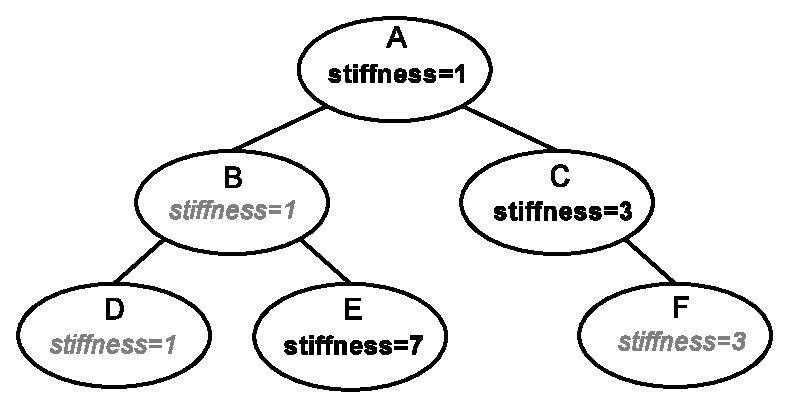
\includegraphics[width=3.75in]{images/inheritedProperties}
\end{center}
\caption{Inheritance of a property named {\it stiffness} among
a component hierarchy. Explicit settings are in bold; inherited settings
are in gray italic.}
\label{inheritedProperties:fig}
\end{figure}

Composite properties are possible, in which a property value is a
composite object that in turn has subproperties. A good example of
this is the {\tt RenderProps} class, which is
associated with the property {\tt renderProps} for renderable objects
and which itself can have a number of subproperties such as {\tt
visible}, {\tt faceStyle}, {\tt faceColor}, {\tt lineStyle}, {\tt
lineColor}, etc.

Properties can be declared to be {\tt inheritable}, so that their
values can be inherited from the same properties hosted by ancestor
components further up the component hierarchy. Inheritable properties
require a more elaborate declaration and are associated with a {\it
mode} which may be either {\tt Explicit} or {\tt Inherited}.  If a
property's mode is inherited, then its value is obtained from
the closest ancestor exposing the same property whose mode is
explicit. In Figure (\ref{inheritedProperties:fig}), the property {\it
stiffness} is explicitly set in components A, C, and E, and inherited
in B and D (which inherit from A) and F (which inherits from C).

\section{Creating an application model}
\label{CreatingAnApplication:sec}

ArtiSynth applications are created by writing and compiling
an {\it application model} that is a subclass of {\tt RootModel}.
This application-specific root model is then loaded and run by the
ArtiSynth program.

The code for the application model should:

\begin{itemize}

\item Declare a no-args constructor

\item Override the {\tt RootModel}
\javamethod*[artisynth.core.workspace.RootModel]{build()}
method to construct the application.

\end{itemize}

ArtiSynth can load a model either using the build method
or by reading it from a file:

\begin{description}

\item[Build method] \mbox{}

ArtiSynth creates an instance of the
model using the no-args constructor, assigns it a name
(which is either user-specified or the simple name of the class), and
then calls the {\tt build()} method to perform the actual
construction.

\item[Reading from a file] \mbox{}

ArtiSynth creates an instance of the
model using the no-args constructor, and then the model is named
and constructed by reading the file.

\end{description}

The no-args constructor should perform whatever initialization is
required in both cases, while the {\tt build()} method takes the place of the
file specification. Unless a model is originally created using a file
specification (which is very tedious), the first time
creation of a model will almost always entail using the {\tt build()}
method.

The general template for application model code looks like this:

\begin{lstlisting}[]
package artisynth.models.experimental; // package where the model resides
import artisynth.core.workspace.RootModel;
... other imports ...

public class MyModel extends RootModel {

   // no-args constructor
   public MyModel() {
      ... basic initialization ...
   }

   // build method to do model construction
   public void build (String[] args) {
      ... code to build the model ....
   }
}
\end{lstlisting}
Here, the model itself is called {\tt MyModel}, and is defined in the
(hypothetical) 
package {\tt artisynth.models.experimental} (placing models in the super
package {\tt artisynth.models} is common practice but not
necessary).

\begin{sideblock}
Note: The {\tt build()} method was only introduced in ArtiSynth
3.1. Prior to that, application models were constructed using a
constructor taking a {\tt String} argument supplying the name of the
model. This method of model construction still works but is
deprecated.
\end{sideblock}

\subsection{Implementing the build() method}
\label{ImplementingBuild:sec}

As mentioned above, the {\tt build()} method is responsible for actual
model construction.  Many applications are built using a single
top-level {\tt MechModel}.  Build methods for these may look
like the following:
\begin{lstlisting}[]
   public void build (String[] args) {
      MechModel mech = new MechModel("mech");
      addModel (mech);

      ... create and add components to the mech model ...
      ... create and add any needed agents to the root model ...

   }
\end{lstlisting}
First, a \javaclass[artisynth.core.mechmodels]{MechModel} is created
(with the name {\tt "mech"} in this example, although any name, or no
name, may be given) and added to the list of models in the root model
using the {\tt addModel()} method. Subsequent code then creates and
adds the components required by the {\tt MechModel}, as described in
Chapters \ref{MechModelsI:sec}, \ref{MechModelsII:sec} and
\ref{FEMModels:sec}.  The {\tt build()} method also creates and adds
to the root model any agents required by the application (controllers,
probes, etc.), as described in Section \ref{SimulationControl:sec}.

Each of the {\tt MechModel} component containers described in
Section \ref{MechModel:sec} is associated with a set of access methods that
allow components to be added, queried, and removed. For example, for
{\tt points}, these include:
%
\begin{methodtable}{0.5}{0.5}
\midline
%
\methodentry
{\mech.MechModel.addPoint()}%
{void addPoint (Point p)}%
{Adds point {\tt p} to the container.}%
%
\methodentry
{\mech.MechModel.removePoint()}%
{boolean removePoint (Point p)}%
{Removes point {\tt p} from the container.}%
%
\methodentry
{\mech.MechModel.clearPoints()}%
{void clearPoints()}%
{Removes all points.}%
%
\methodentry
{\mech.MechModel.points()}%
{PointList<Point> points()}%
{Returns the point container.}%
%
%\methodspace{0.5em}%
%\brh
\midline
\end{methodtable}
%
A component container itself is iterable, and also supplies the methods {\tt
size()} and {\tt get(int i)} that return the number of components and the
$i$-th component in the container. For example, the following code fragment
shows two ways to iterate through the points in the {\tt points} container:
%
\begin{lstlisting}[]
  MechModel mech;
  ...
  PointList<Point> points = mech.points();
  for (int i=0; i<points.size(); i++) {
     Point p = points.get(i);
     ... do something with p ...
  }
  ...
  for (Point p : mech.points()) {
     ... do something with p ...
  }
\end{lstlisting}
%
\begin{sideblock}
While a component container also contains {\tt add()} and {\tt remove()}
methods, it is generally recommended that these not be used for modifying the
contents of the default containers.
\end{sideblock}

\begin{sideblock}
Applications do {\it not} have to use the default component containers.
Instead, they may create their own custom containers, as described in
Section \ref{GeneralComponentArrangements:sec}.
\end{sideblock}

When constructing a model, there is no fixed order in which components need to
be added. For instance, in the above example, {\tt addModel(mech)} could be
called near the end of the {\tt build()} method rather than at the
beginning. However, all components needed for the simulation must be added {\it
somewhere} to the {\tt MechModel} component hierarchy during the build process.
This includes any components referenced by other components. For instance,
an axial spring (Section \ref{ParticlesAndSprings:sec}) refers to two
points. If either of these points have not been added to the hierarchy,
an exception similar to the following will be raised after the {\tt build()}
method exits:
%
\begin{lstlisting}[]
java.lang.IllegalStateException: Particle p2 referenced by AxialSpring 
   ParticleSpring/models/mech/axialSprings/spr is outside containment hierarchy
\end{lstlisting}
%

The {\tt build()} method supplies a {\tt String} array as an argument,
which can be used to transmit application arguments in a manner
analogous to the {\tt args} argument passed to static {\tt main()}
methods. Build arguments can be specified when a model is loaded
directly from a class using {\sf Models > Load from class ...}, or when
the {\it startup model} is set to automatically load a model
when ArtiSynth is first started ({\sf Settings > Startup
model}). Details are given in the ``Loading, Simulating and
Saving Models'' section of the
\artisynthManual{uiguide}{User Interface Guide}.

Build arguments can also be listed directly on the ArtiSynth command
line when specifying a model to load using the {\tt -model
<classname>} option.  This is done by enclosing the desired arguments
within square brackets {\tt [ ]} immediately following the {\tt
-model} option. So, for example,
%
\begin{verbatim}
> artisynth -model projects.MyModel [ -size 50 ]
\end{verbatim}
%
would cause the strings {\tt "-size"} and {\tt "50"} to
be passed to the {\tt build()} method of {\tt MyModel}.

\subsection{Making models visible to ArtiSynth}

In order to load an application model into ArtiSynth, the classes
associated with its implementation must be made visible to ArtiSynth.
This usually involves adding the top-level class folder associated
with the application code to the classpath used by ArtiSynth.

\begin{sideblock}
The demonstration models referred to in this guide belong to the
package {\tt artisynth.demos.tutorial} and are already visible to
ArtiSynth.
\end{sideblock}

In most current ArtiSynth projects, classes are stored in
a folder tree separate from the source code, with the top-level
class folder named {\tt classes}, located one level below
the project root folder. A typical top-level class folder
might be stored in a location like this:
\begin{verbatim}
  /home/joeuser/artisynthProjects/classes
\end{verbatim}
In the example shown in Section \ref{CreatingAnApplication:sec}, the
model was created in the package {\tt artisynth.models.experimental}.
Since Java classes are arranged in a folder structure that mirrors
package names, with respect to the sample project folder shown
above, the model class would be located in
\begin{verbatim}
  /home/joeuser/artisynthProjects/classes/artisynth/models/experimental
\end{verbatim}

At present there are three ways to make top-level class folders
known to ArtiSynth:

\begin{description}

\item[Add projects to your Eclipse launch configuration]\mbox{}

If you are using the Eclipse IDE, then you can add the project in
which are developing your model code to the launch configuration that
you use to run ArtiSynth. Other IDEs will presumably provide similar
functionality.

\item[Add the folders to the external classpath]\mbox{}

You can explicitly add the class folders to ArtiSynth's external
classpath. The easiest way to do this is to select ``{\sf Settings >
External classpath ...}'' from the {\sf Settings} menu, which will
open an external classpath editor which lists all the classpath
entries in a large panel on the left. (When ArtiSynth is first
installed, the external classpath has no entries, and so this panel
will be blank.) Class folders can then by added via
the {\sf ``Add class folder''} button, and the classpath is
saved using the {\sf Save} button.

\item[Add the folders to your CLASSPATH environment variable]\mbox{}

If you are running ArtiSynth from the command line, using the {\tt
artisynth} command (or {\tt artisynth.bat} on Windows), then you can
define a CLASSPATH environment variable in your environment and add
the needed folders to this.

\end{description}

All of these methods are described in more detail in the ``Installing
External Models and Packages'' section of the ArtiSynth Installation
Guide (available for 
\artisynthManual[installation/linuxInstallation]{linuxInstallation}{Linux}, 
\artisynthManual[installation/windowsInstallation]{windowsInstallation}{Windows},
and 
\artisynthManual[installation/macosInstallation]{macosInstallation}{MacOS}).

\subsection{Loading and running a model}
\label{LoadingAndRunning:sec}

If a model's classes are visible to ArtiSynth, then it may be loaded
into ArtiSynth in several ways:

\begin{description}

\item[Loading from the Model menu]\mbox{}

If the root model is contained in a package located under {\tt
artisynth.demos} or {\tt artisynth.models}, then it will appear in the
default model menu ({\sf Models} in the main menu bar) under the
submenu {\sf All demos} or {\sf All models}.

\item[Loading by class path]\mbox{}

A model may also be loaded by choosing {\sf ``Load from class ...''}
from the {\sf Models} menu and specifying its package name and then
choosing its root model class. It is also possible to use the {\tt
-model <classname>} command line argument to have a model loaded
directly into ArtiSynth when it starts up.

\item[Loading from a file]\mbox{}

If a model has been saved to a {\tt .art} file, it may be loaded from
that file by choosing {\sf File > Load model ...}.

\end{description}

These methods are described in detail in the 
section ``Loading and Simulating Models'' of the\pdfbreak
\artisynthManual{uiguide}{ArtiSynth User Interface Guide}.

\begin{sideblock}
The demonstration models referred to in this guide should already
be present in the model menu and may be loaded
from the submenu {\sf Models > All demos > tutorial}.
\end{sideblock}

Once a model is loaded, it can be simulated, or {\it run}.  Simulation
of the model can then be started, paused, single-stepped, or reset
using the play controls (Figure \ref{PlayControlsFig}) located at the
upper right of the ArtiSynth window frame.  Starting and stopping a
simulation is done by clicking {\sf play/pause}, while {\sf reset}
resets the simulation to time 0.  The {\sf single-step} button
advances the simulation by one time step. The {\sf stop-all} button
will also stop the simulation, along with any Jython commands or
scripts that are running.

\begin{figure}[ht]
\begin{center}
\iflatexml

\includegraphics[]{../uiguide/images/playControls}
\else

\includegraphics[width=3in]{../uiguide/images/playControls}
\fi
\end{center}
\caption{The ArtiSynth play controls. From left to right: step size
control, current simulation time, and the reset, skip-back,
play/pause, single-step, skip-forward and stop-all buttons.}%
\label{PlayControlsFig}
\end{figure}

Comprehensive information on exploring and interacting with models is
given in the
\artisynthManual{uiguide}{ArtiSynth User Interface Guide}.

\ifdefined\maindoc
\else
\end{document}
\fi
